
\chapter{相关工作}

\section{相关的理论研究工作}

\subsection{利用社区提高开源软件质量}

\subsection{自动性能分析}

\section{相关工程项目}

Linux内核作为一个庞大和复杂的系统软件,很早之前就已经引起了很多公司或团体的注意,并以之为测试目标,开发了比较实用,比较方便的进行Linux性能测试的工程项目,比如LKP\cite{chen2007keeping}和MMTests就是其中两个比较优秀的项目。

\subsection{Linux Kernel Performance}

Linux Kernel Performance(简称LKP),是Intel公司的开源技术中心于2005年开始的一个用于进行Linux内核性能测试的一个测试框架。

由于Linux内核的快速发展,Intel开源技术中心的一部分工程师开发了一套对Linux内核性能进行测试的框架,这套框架的具体架构如图\ref{fig:old_lkp_arch}

\begin{figure}[H]
\centering
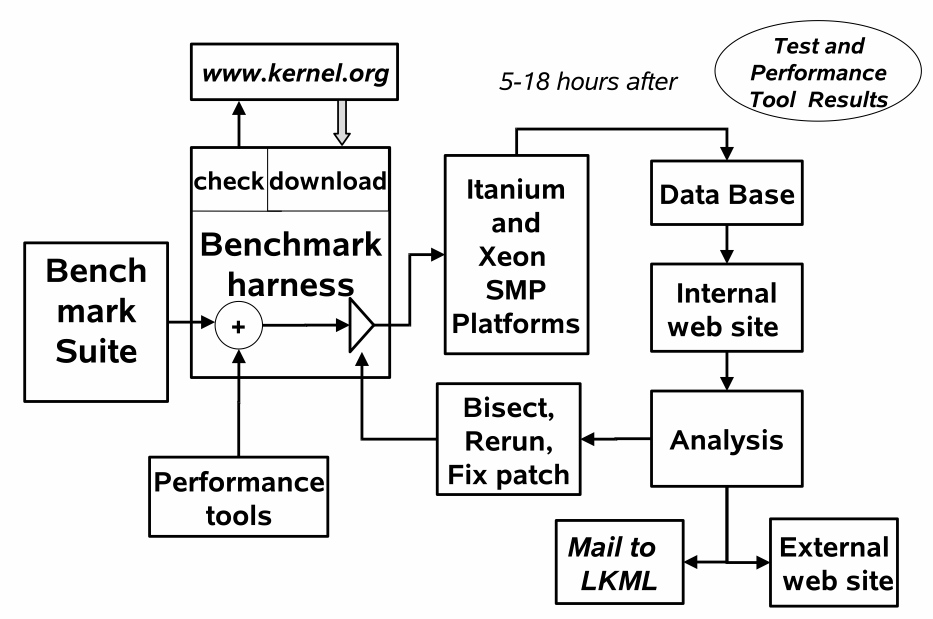
\includegraphics[width=10cm]{old_lkp_arch}
\caption{LKP测试框架架构}
\label{fig:old_lkp_arch}
\end{figure}

在这套框架中,主要的测试分为5个阶段,分别是:
\begin{enumerate}
\item 下载代码并编译。首先从linux.org网站上面下载各个版本的内核源代码,并进行编译,一般都只是对具有tag的版本(包括RC版本和最终发行版)进行编译。
\item 运行测试。使用上一个阶段中编译好的内核来启动一台物理机器,并在这一台物理机器中运行各种各样的测试例程,如Kbuild,Reaim7,Netperf,Tbench等比较经典和常用的测试例程。同时,在测试例程运行的过程中,还会启动vmstat,iostat,sar,ps等工具来进行测试数据的采样和收集,采集到的数据都将被保存在数据库中,方便在后来进行查询。
\item 结果分析。根据在上一个阶段中收集到的测试数据,作出相关的数据统计分析,同时结合每一个测试例程的运行结果来给每一次的测试进行评分。在评分的过程中,给予每一个不同的测试例程相应的权重值,然后根据权重值计算出本次测试的得分,然后通过得分来判定性能的变化情况。
\item 问题查找。如果在进行结果分析的时候发现了性能回退的情况,那么就会在Linux内核的代码树中使用git-bisect来进行问题的查找,定位出问题发生的位置和原因,然后将问题的定位和分析结果通过邮件的形式发送给Linux内核的邮件列表中。
\item 结果呈现。将测试的结果通过不同的形式展示出来,在LKP中提供一个web界面进行测试数据的浏览,数据会以表格或者图表的形式进行展示,方便开发者们查看数据变化的趋势。
\end{enumerate}

在任何的测试系统中,测试时的波动都是需要考虑的内容,在LKP中同样也不例外。

LKP中对测试时发生的波动的处理可以说是比较简单,但是同样也是比较有效的,其中采用的具体措施有以下几个:
\begin{enumerate}
\item 每次都在一个已知的系统状态上开始测试
\item 在进行正式的测试之前,会使用一些简单的测试例程来使得系统到达一个比较稳定的状态
\item 通过进行长时间的测试以及多次运行测试例程后取平均值来得到最终的测试结果
\end{enumerate}

然而,这样的措施虽然能够在一定的程度上降低测试波动造成的影响,并能够检测到一些比较严重的性能回退问题,但是一些较小的性能回退仍然有可能会混淆在测试的波动中。

\subsection{MMTests}